%!TEX root = main.tex
%
\section{Research Method}
\subsubsection{Design as an artifact}
By definition, the result of design-science research in Information Science is:
\begin{quote}
\emph{A purposeful IT artifact created to address an important organizational problem. It must be described effectively, enabling its implementation and application in an appropriate domain.} \citep{Esearch2004}
\end{quote}
Markus et al.\citep{markusetal} identified that a developed artifact is only significant by looking at some significant questions: 
\begin{itemize}
\item Can the artifact be constructed?
\item Can the artifact perform appropriately?
\item Is the result important to the information science community?
\end{itemize}
We will create a proof of concept prototype tool for promoting reflection on work experiences experienced, by utilizing project artifacts collected from version-control systems. Our goal was to create a tool that can discover new capabilities in the domain of reflection on experiences and learning from these, as well as support the existing capabilities in an efficient way. Evaluating the tool in \emph{real use} situations is necessary in order to discover if the artifact can enhance the reflection process as it is today.

\subsubsection{Research Guidelines}
The \emph{Design-Science Research Guidelines} presented in \citep{Esearch2004} will serve as the basis of this design-science research. The guidelines were created in order to assist researchers to understand the necessary requirements for effective design-science research. 

\subsection{Design as a research process}
Development of the application was done in development cycles, inspired be the regulative cycle presented by Wieringa \citep{wieringa}, and is shown in Figure ~\ref{regulativecycle}. The development process and the regulative cycle we adopted for developing the application is further detailed in Section \ref{subsec:devprocess} and Section \ref{sec:dailydeliverycycle}.
The early parts of the development process was used to develop ideas and basic mock-ups of the application and its design. The initial prototype design was based heavily on the first concept and mock-ups created, in addition to recurring feedback from users and our supervisor. Early parts of development resulted in a prototype with functionality for individual reflection use. The next goal was to incorporate teams and support collaborative reflection in the team, building and improving on the basic functionality present in the tool. In the later parts of the development, the focus was the integration of individual reflection notes, into the team collaborative areas. This resulted in a tool for both individual and collaborative aspects for reflection and learning from experiences. We used the tool ourselves during development, as it would be used in a real working environment. In this way we ensure that all functionality is as expected, and also identify limitations early in the design. 

Finally we performed three different evaluations. First we conducted a usability test with computer-science students, and also an expert review with an expert in the field of agile software development. The last evaluation we conducted was a focus group evaluation with an agile software development team using GitHub as their main version-control system. Evaluating these separately provided three sets of feedback which we could compare in order to possibly see if any patterns emerged.

\begin{figure}[!htpb]
\centering
	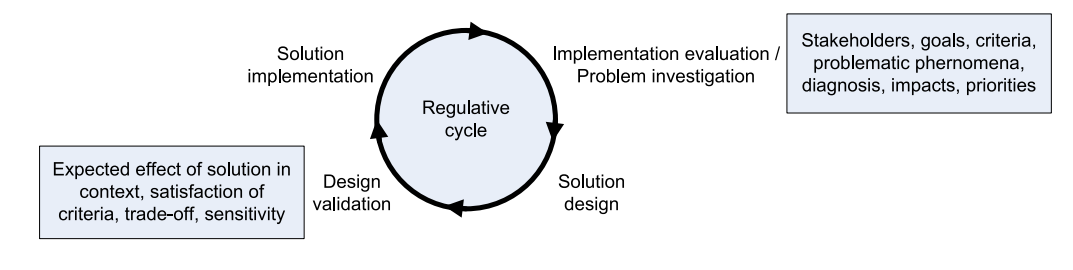
\includegraphics[width=\textwidth]{regulativecycle}
\caption{Regulative cycle development in Design-Science research \citep{wieringa}}
\label{regulativecycle}
\end{figure}

\subsection{Development process}
\label{subsec:devprocess}
\begin{figure}[!htpb]
\centering
	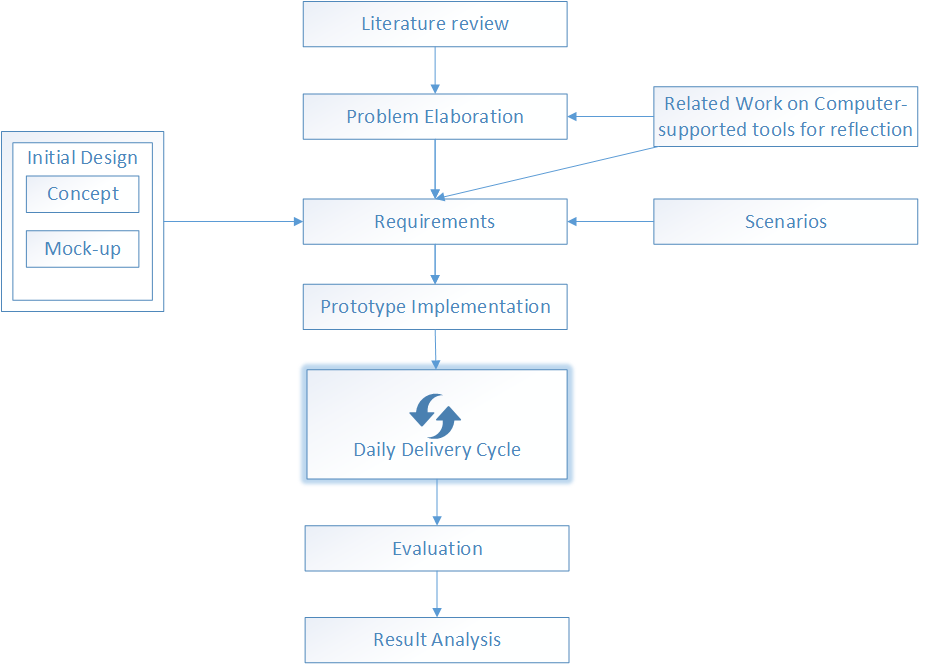
\includegraphics[width=\textwidth]{researchmodel_and_iterationcycle}
\caption{The PeacefulBanana research model }
\label{researchmodel}
\end{figure}

Figure \ref{researchmodel} shows the research model used for the development of our prototype from initial concept and ideas, to the final implementation and evaluation. The model depicts how we started the process by reading theory(top part of model) in order to get a better understanding of the core concepts of reflection on experiences(See Chapter \ref{chap:background} for the thesis background).
\clearpage 
We conducted a literature review (Section \ref{sec:literaturereview}) and looked at related work done on computer-supported tools for reflection and GitHub related tools (Section \ref{sec:relatedwork}). This gave us a basis on which to build a problem elaboration on(See Chapter \ref{chap:problemelaboration}) and this stage can be seen as the second from the top in Figure \ref{researchmodel}. The problem elaboration with our application scenarios, in addition to related tools, led us in turn to the process of creating the requirements for the application (See Chapter \ref{chap:requirements}). The initial design stage to the left in the model, with the application concept and mock-ups also helped further identify requirements for the application, together with feedback from our supervisor. \\
Based on the stages from literature review to requirements in the model shown in Figure \ref{researchmodel}, we started implementing the PeacefulBanana application. These implementations were conducted using a daily delivery cycle, which we used throughout the development phase of the application. This cycle is further described in Section \ref{sec:dailydeliverycycle}. \\
The last two stages of our research model is Evaluation and Result analysis. Evaluation consisted of a usability study, an expert review and a focus group (See Chapter \ref{cha:evaluation}). Based on the findings from these evaluations we were able to perform a result analysis. 

\subsection{Daily Delivery Cycle}
\label{sec:dailydeliverycycle}
Figure\ref{iterationprocess} shows an illustration of the daily delivery cycle used throughout development. This daily delivery cycle was inspired by the regulative cycle presented by Wieringa\citep{wieringa}, shown in Figure \ref{regulativecycle}. How this cycle fits in the overall stages of research is shown in Figure \ref{researchmodel}.
\begin{figure}[!htpb]
\centering
	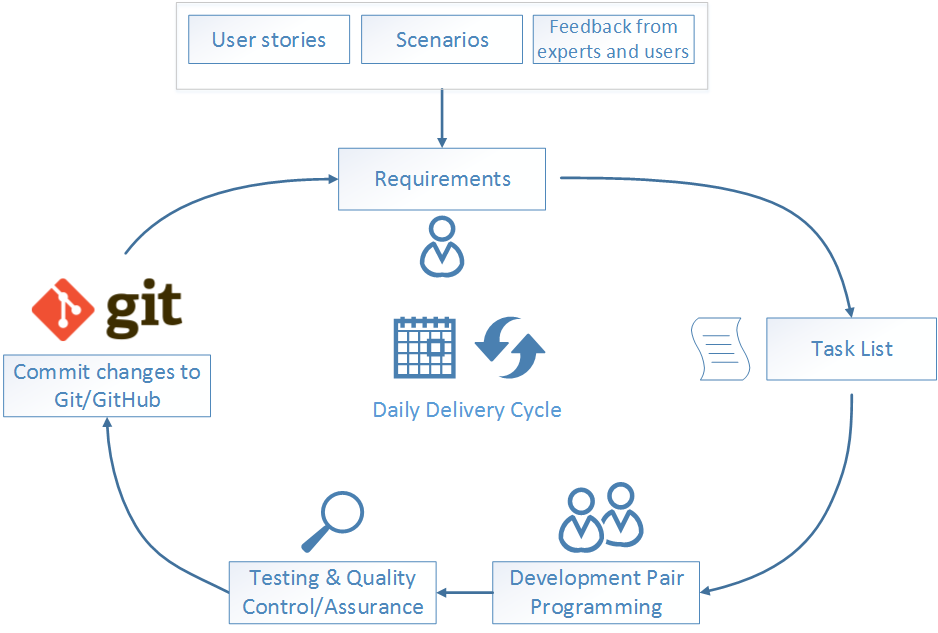
\includegraphics[width=\textwidth]{iterationprocess}
\caption{The PeacefulBanana daily delivery cycle}
\label{iterationprocess}
\end{figure}

The cycle starts with a set of requirements. These requirements are initially based on user-stories and scenarios. In subsequent iterations of the cycle, the requirements were then updated based on feedback from from experts and users of the application. A task list is then created from the set of requirements, where the highest prioritized requirements was implemented first. This task list acts as a backlog 
\footnote{The backlog is the list of work the developers must address during the current iteration} for the application. On GitHub we created the more general tasks as \emph{Milestones} and the more specific tasks as \emph{Issues} connected to these milestones\footnote{GitHub Issues \& Milestones: \url{https://github.com/features/projects/issues}}.

Development was conducted primarily using pair-programming\footnote{Pair programming is an agile software development technique in which two programmers work together at one workstation}, so that we could review each line of code as it was written. Whenever a task implementation was completed, it was tested manually in the application, as well as by automatic tests. When a feature was accepted and working as intended, we submitted the code to our project repository on GitHub.
This ensured an iterative approach to development, expanding our application with more and more quality-assured functionality. 

\subsubsection*{Dogfooding}
\label{dogfooding}
While developing the application, we continuously used the application ourselves, this is a concept called dogfooding.

Dogfooding is a concept where you 'eat your own dog food', this means that the developers are testing their own product while developing it\citep{dogfooding}. It is normally something larger software development teams are doing as a pre alpha-testing, this will help developers to discover eventual problem-areas early.
\clearpage

\subsection{Evaluation} 
The table shown in Figure \ref{table2evaluation} from \citep{Esearch2004} serve as guidelines for the different evaluations of the application. The evaluations and the results from these are further described in Chapter \ref{cha:evaluation}. During the final focus group evaluation we also made use of the evaluation toolbox published by MIRROR\footnote{\url{http://www.mirror-project.eu/showroom-a-publications/downloads/finish/5/67}}. This toolbox is a specification of evaluation methodology and research tooling. 
\begin{figure}[H]
\centering
	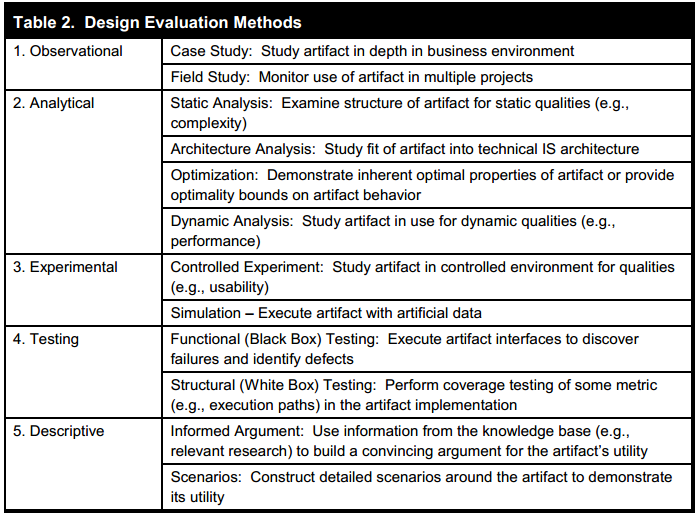
\includegraphics[width=\textwidth]{table2evaluation}
\caption{Design Evaluation Methods}
\label{table2evaluation}
\end{figure}
\begin{enumerate}
	\item \textbf{Observational}: Both in the usability study and the focus group evaluation we provided participants with a set of questions where they evaluate the application. In the focus group evaluation we provided participants with application specific questions and the reflection scale from the MIRROR toolbox [Appendix \ref{reflectionscale}]. The reflection scale assesses participants' general tendency to reflect and the importance they place on reflection. Using this scale, allows us to see whether using the tool prime people to reflect more, that is: Does the tool increase the users tendency to reflect on experiences, both individually and as a team.
	\item \textbf{Analytical}: A separate administration interface were implemented in order to collect data usage statistics from users. These data could provide simple usage-patterns during i.e. a future case-study of a development team using the application. Examples of these data can be seen in Figure: \ref{notestatistics} and  \ref{githubstatistics}. Having such data might also provide a basis for an analysis of the application's performance as well as it's usefulness in the domain of reflection in software development teams. 
	\item \textbf{Experimental}: we performed a usability study as a controlled experiment (See Section \ref{sec:usabilityeval}).
	\item \textbf{Testing}: During development we continuously tested the tool to ensure that the user experience is as expected, as a means of quality assurance. White Box testing were used during development of the application with artificial data to ensure functions are working properly and as specified. 
	\item \textbf{Descriptive}: In order to demonstrate the usefulness of our application we constructed two detailed scenarios, demonstrating it's use for tasks in a real work environment (See Chapter \ref{chap:problemelaboration}, Section \ref{sec:scenarios}). All three evaluations used the context of these scenarios to evaluate the application and provide feedback. In addition to these evaluations we have continuously used the application ourselves in order to identify any problems as we develop the application (See Section \ref{dogfooding}).
\end{enumerate}
\begin{figure}[!htpb]
\centering
	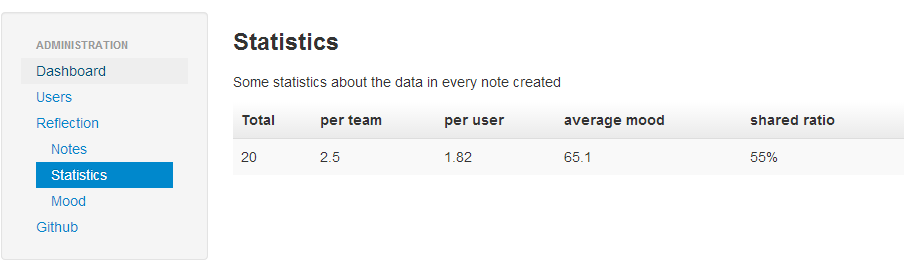
\includegraphics[width=\textwidth]{notestatistics}
\caption{Reflection note statistics}
\label{notestatistics}
\end{figure}
\begin{figure}[!htpb]
\centering
	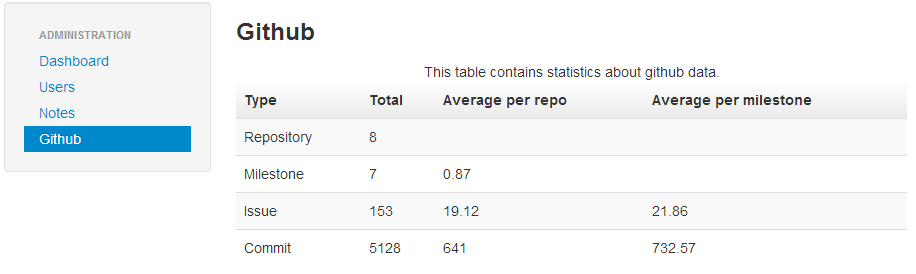
\includegraphics[width=\textwidth]{githubstatistics}
\caption{GitHub statistics}
\label{githubstatistics}
\end{figure}

\subsection{Research Contributions}
The main goal was to create a proof of concept application that may help users reflect on their past experiences, both individually and collaboratively in reflection sessions, by collecting experiences daily, storing and revisiting them at any time. The implementation of the application and the evaluation of it gave us a foundation to answer our research questions, and also identify areas that can go into future research and development in the domain of technology supported reflection and collaboration. 
Future work  and the identified proposed features and improvements can be seen in Section \ref{sec:futurework}
 will provide an increased understanding of how technology can support reflection in software development teams, by collecting and revisiting experiences from everyday work. 

\subsection{Research Rigor}
The application was evaluated through a usability test, an expert review with an expert in the field of agile software development and a focus group consisting of a software development team. By evaluating the application with experts in the relevant fields provides an indication for the usefulness of the application.

\subsection{Research communication}
The proof of concept application have been released under the GNU Public License v3\footnote{\url{http://www.gnu.org/licenses/gpl.html}} and the repository are located at GitHub: 
\begin{itemize}
	\item \url{https://github.com/ekun/PeacefulBanana}
\end{itemize} 
Any limitations identified  will be documented along with the research results. 



